\chapter{VHDL} % Main chapter title
\label{VHDL} % For referencing the chapter elsewhere, use \ref{Chapter1} 

%----------------------------------------------------------------------------------------
\section{Einleitung}
VHDL (\textit{Very High Speed Integrated Circuit Hardware Description Language}) ist eine Hardwarebeschreibungssprache, die 1980 entwickelt wurde. Mit ihr kann das Verhalten einer logischen Schaltung formal beschrieben werden. \cite[S. 22f.]{kesel2013entwurf}

Anstatt eine Schaltung aus ihren einzelnen elektronischen Bauteilen zu entwerfen, arbeitet VHDL aber auf einer höheren Abstraktionsschicht. Es wird lediglich beschrieben, wie sich eine Schaltung oder ein logischer Teil einer Schaltung in Abhängigkeit bestimmter Eingangsgrößen verhält. Die konkrete technische Umsetzung der Hardware wird damit vom Entwickler abgekapselt.
%----------------------------------------------------------------------------------------

%----------------------------------------------------------------------------------------
\section{Entwicklung mit VHDL}
\paragraph{Entities.} In VHDL werden \textit{Entities} definiert, die eine Klasse von Schaltelementen repräsentieren. Entities bestehen üblicherweise aus mehreren Ein-und Ausgangs\textit{ports}. Innerhalb einer Entity wird ihre \emph{Architecture} beschrieben. Diese kann entweder ihr Verhalten als innere Funktion oder ihre Struktur beschreiben.

\paragraph{Architecture.} Im \emph{Verhaltensmodell} einer Entity wird definiert, wie sich die Ausgangssignale in Abhängigkeit der Eingangssignale verhalten. Dafür können die Eingangssignale direkt oder über kombinatorische Schaltungen an die Ausgänge weitergeleitet werden. 

Um komplexe Schaltungen hierarchisch zu gliedern, kann die Architecture auch als \emph{Strukturmodell} beschrieben werden. Hier wird auf übergeordneter Ebene die Verschaltung mehrerer Subkomponenten definiert. Dafür werden Instanzen von zuvor beschriebenen Entities (sog. \textit{Components}) erstellt und deren Ports miteinander verbunden. \cite[S. 25ff.]{kesel2013entwurf}

\paragraph{Prozesse.} Bei der Entwicklung ist insbesondere zu beachten, dass das Verhalten einer Entity, anders als von Programmiersprachen gewohnt, im Allgemeinen nicht sequentiell abgearbeitet wird. Vielmehr findet die Signalverarbeitung grundsätzlich parallel statt. Im Verhaltensmodell einer Entity können deshalb Prozesse deklariert werden, deren Instruktionen sequentiell abgearbeitet werden. Innerhalb eines Prozesses können dann auch \textit{Variablen} verwendet werden, die sich vergleichbar mit Variablen von Programmiersprachen verhalten. \cite[S. 29f.]{kesel2013entwurf}
%----------------------------------------------------------------------------------------
 
%----------------------------------------------------------------------------------------
\section{Umsetzung von VHDL}
Auf die konkrete Umsetzung der beschriebenen Schaltung hat der Anwender selbst nur bedingten Einfluss, da die Implementierung der Schaltung in Hardware üblicherweise von automatisierten Werkzeugen durchgeführt wird. Dabei lassen sich mehrere Schritte unterscheiden. In diesem Projekt wurde die Entwicklungsumgebung Vivado Design Suite von Xilinx verwendet, um den VHDL-Code umzusetzen.

\paragraph{Simulation.} In einem ersten Schritt kann das Verhalten des VHDL Codes \emph{simuliert} werden, was vor allem in der Testphase von Bedeutung ist. Dabei wird der Code noch nicht auf der Hardware ausgeführt, sondern das Verhalten der Schaltung mittels sogenannter Testbenches simuliert, die die Schaltung mit virtuellen Eingangssignalen (z. B. Taktrate) versorgt. \cite[S. 81]{SynthesisFPGA} Der Quellcode der verwendeten Haupttestbench dieses Projekts ist in im Anhang \ref{src:main_tb.vhd} zu sehen. 

\begin{figure} [ht]
  \centering
  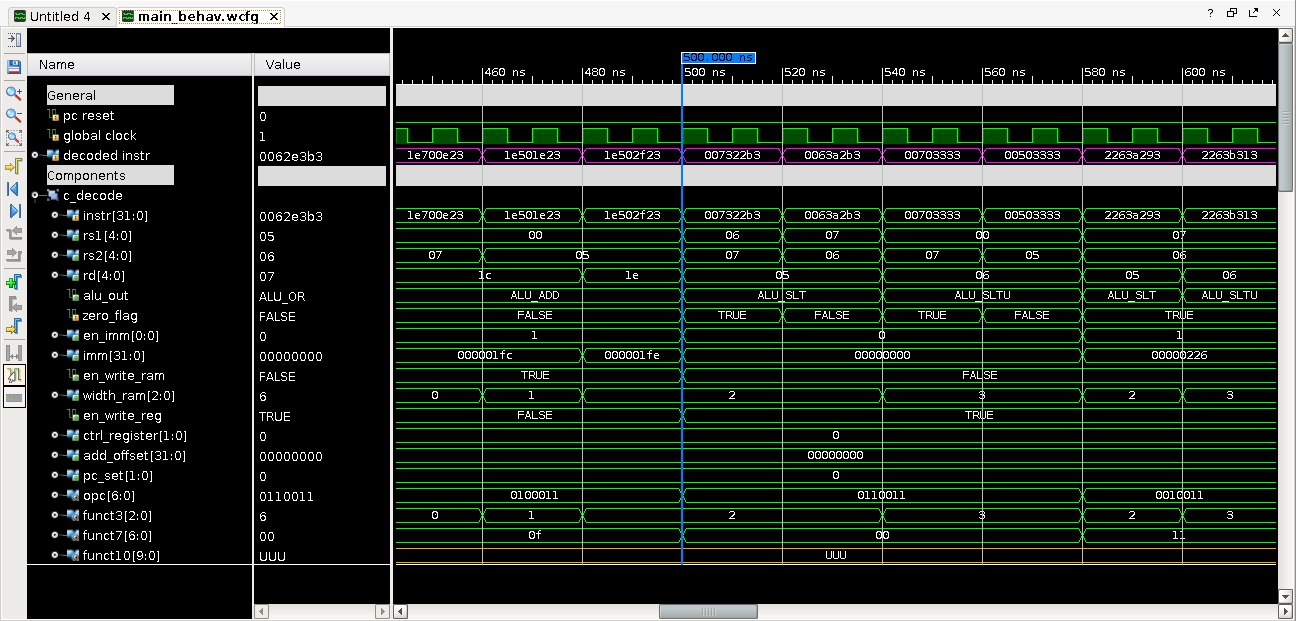
\includegraphics[width=\textwidth]{Figures/simulation}
  \caption{Beispiel für die Simulation einer komplexen Schaltung mit Vivado Design Suite: Zu sehen ist die graphische Darstellung von Signalen in Abhängigkeit der Zeitkomponente}
  \label{fig:simulation}
\end{figure}

\paragraph{Synthese.} Das simulierte Verhalten kann anschließend \emph{synthetisiert} werden. Dabei ist zu beachten, dass nicht die vollständige Menge von zulässigem (und simulationsfähigem) VHDL-Code letztlich in eine physische Schaltung synthetisierbar ist (so z. B. \emph{wait}-Statements). Das ist abhängig von der verwendeten Zieltechnologie (FPGA, ASIC) und dem verwendeten Synthesewerkzeug. Das Ergebnis der Synthese ist eine (hardwareunabhängige) Netzliste, die einer textuellen Beschreibung des umgesetzten Schaltplans entspricht.

\paragraph{Implementierung.} Diese Netzliste ist Grundlage der Hardwareimplementierung. Dabei wird innerhalb des \emph{place and route} Vorgangs unter Berücksichtigung der verfügbaren Hardware und bestimmter zeitlicher Beschränkungen berechnet, wo die einzelnen Schaltelemente auf der Hardware implementiert werden und wie sie verbunden werden. In diesem Schritt wird ein Bitstream generiert, der anschließend auf die Hardware geladen werden kann. \cite[S. 21]{SynthesisFPGA}
%----------------------------------------------------------------------------------------
